%==================== PARTIE 3 ====================
\section{Partie 3 : Débruitage d'un signal audio}

Le signal de référence $d(n)$ est un enregistrement d'ambiance de plage (vagues et chants d'oiseaux), lu dans \texttt{monson.wav} ($F_s=44100$~Hz). On garde un canal et $N=10^5$ échantillons ($\approx 2.27$~s), en sautant la première seconde (silence). Le bruitage est celui de la partie~2 : $x(n)=d(n)+v(n)$, $v(n)\sim\mathcal{N}(0,\sigma_v^2)$, avec \texttt{rng(0)} pour des résultats reproductibles.

\textbf{Normalisation.} Le signal brut est très faible ($P_d\approx 0.0016$) : avec $\sigma_v^2=0.1$, le bruit serait 60 fois plus puissant et le filtre rendrait une sortie quasi nulle ($\mathrm{EQM}_{\min}=0.0015\approx P_d$). On normalise donc : $d(n)\leftarrow d(n)/\max|d(n)|$, comme la sinusoïde de la partie~2.

\subsection{Question préliminaire : RSB de 0 dB}

\begin{enonce}
\textbf{Énoncé :} Quelle valeur de $\sigma_v^2$ permet d'avoir un RSB avant débruitage de 0~dB ?
\end{enonce}

\textbf{Démarche.}
\[
\mathrm{RSB}_{\mathrm{av}}=10\log_{10}\frac{P_d}{\sigma_v^2}=0~\text{dB}
\iff \sigma_v^2=P_d=r_d(0)=\frac{1}{N}\sum_{n=1}^{N}d^2(n).
\]

\textbf{Code.}
\begin{lstlisting}
clear; clc; close all;
rng(0);                              % bruit reproductible

[y, Fs] = audioread('monson.wav');   % lecture du son
y = y(:,1);                          % un seul canal

N     = 1e5;
debut = round(1*Fs);                 % on saute la 1re seconde
d = y(debut+1 : debut+N);            % signal de reference
d = d / max(abs(d));                 % normalisation dans [-1, 1]

% Puissance du signal r_d(0)
Sd = 0;
for k = 1:N
    Sd = Sd + d(k)^2;
end
Pd = Sd / N;
fprintf('Pd = %.4f -> sigma_v^2 pour RSB = 0 dB : %.4f\n', Pd, Pd);
\end{lstlisting}

\begin{resultat}
$P_d=0.0411$, donc $\boldsymbol{\sigma_v^2=0.0411}$ donne un RSB de 0~dB.
\end{resultat}

\begin{interpretation}
La puissance du signal audio normalisé est 12 fois plus faible que celle de la sinusoïde ($0.5$) : il reste la plupart du temps proche de zéro, avec quelques pics. Avec $\sigma_v^2=0.1$, le RSB de départ est donc négatif.
\end{interpretation}

\subsection{Question (a) : \texorpdfstring{$\mathrm{EQM}_{\min}$ pour $P=10$ et $\sigma_v^2=0.1$}{EQMmin pour P = 10}}

\begin{enonce}
\textbf{Énoncé :} Afin d'évaluer la performance du débruitage, calculer $\mathrm{EQM}_{\min}=r_d(0)-\mathbf{w}_{opt}^T\mathbf{r}_{dx}$ pour $P=10$ et $\sigma_v^2=0.1$.
\end{enonce}

\textbf{Démarche.} Bruitage, calcul de $\mathbf{w}_{opt}$ et de $\hat d(n)$ comme en partie~2, puis de $\mathrm{EQM}_{\min}$. Pour juger la performance, on la compare à l'erreur sans filtrage ($\sigma_v^2$) et à l'erreur d'une sortie nulle ($P_d$), et on calcule le gain $\mathrm{gain}|_{\mathrm{dB}}=10\log_{10}(P_d/\mathrm{EQM}_{\min})-10\log_{10}(P_d/\sigma_v^2)$.

\textbf{Code.} (à la suite du code précédent)
\begin{lstlisting}
P = 10;  sigv2 = 0.1;

x = d + sqrt(sigv2)*randn(N,1);      % signal bruite

% Filtre de Wiener : r_dx(k) = r_d(k)
rx = xcorr(x, P-1, 'biased'); rx = rx(P:end);
rd = xcorr(d, P-1, 'biased'); rd = rd(P:end);
wopt = toeplitz(rx) \ rd;
dhat = filter(wopt, 1, x);           % signal debruite

% EQM minimale (rd(1) correspond a r_d(0))
EQMmin = rd(1) - wopt'*rd;
fprintf('EQM_min = %.4f (bruit avant filtrage : %.2f)\n', EQMmin, sigv2);

% RSB avant / apres et gain
RSB_av = 10*log10(rd(1)/sigv2);
RSB_ap = 10*log10(rd(1)/EQMmin);
fprintf('RSB avant = %.2f dB | RSB apres = %.2f dB | gain = %.2f dB\n', ...
        RSB_av, RSB_ap, RSB_ap - RSB_av);

% Affichage d'une fenetre
idx = 1001:1300;
figure;
plot(idx, x(idx), 'Color', [0.7 0.7 0.7]); hold on;
plot(idx, d(idx), 'b', 'LineWidth', 1.2);
plot(idx, dhat(idx), 'r', 'LineWidth', 1.2);
grid on; xlabel('n'); ylabel('Amplitude');
legend('x(n) : signal bruite', 'd(n) : signal propre', ...
       'dhat(n) : signal debruite');
saveas(gcf, 'figs_partie3/p3_qa_signaux.png');

% Ecoute
sound(d, Fs);    pause(N/Fs + 0.5);
sound(x, Fs);    pause(N/Fs + 0.5);
sound(dhat, Fs);
\end{lstlisting}

\begin{figure}[H]
  \centering
  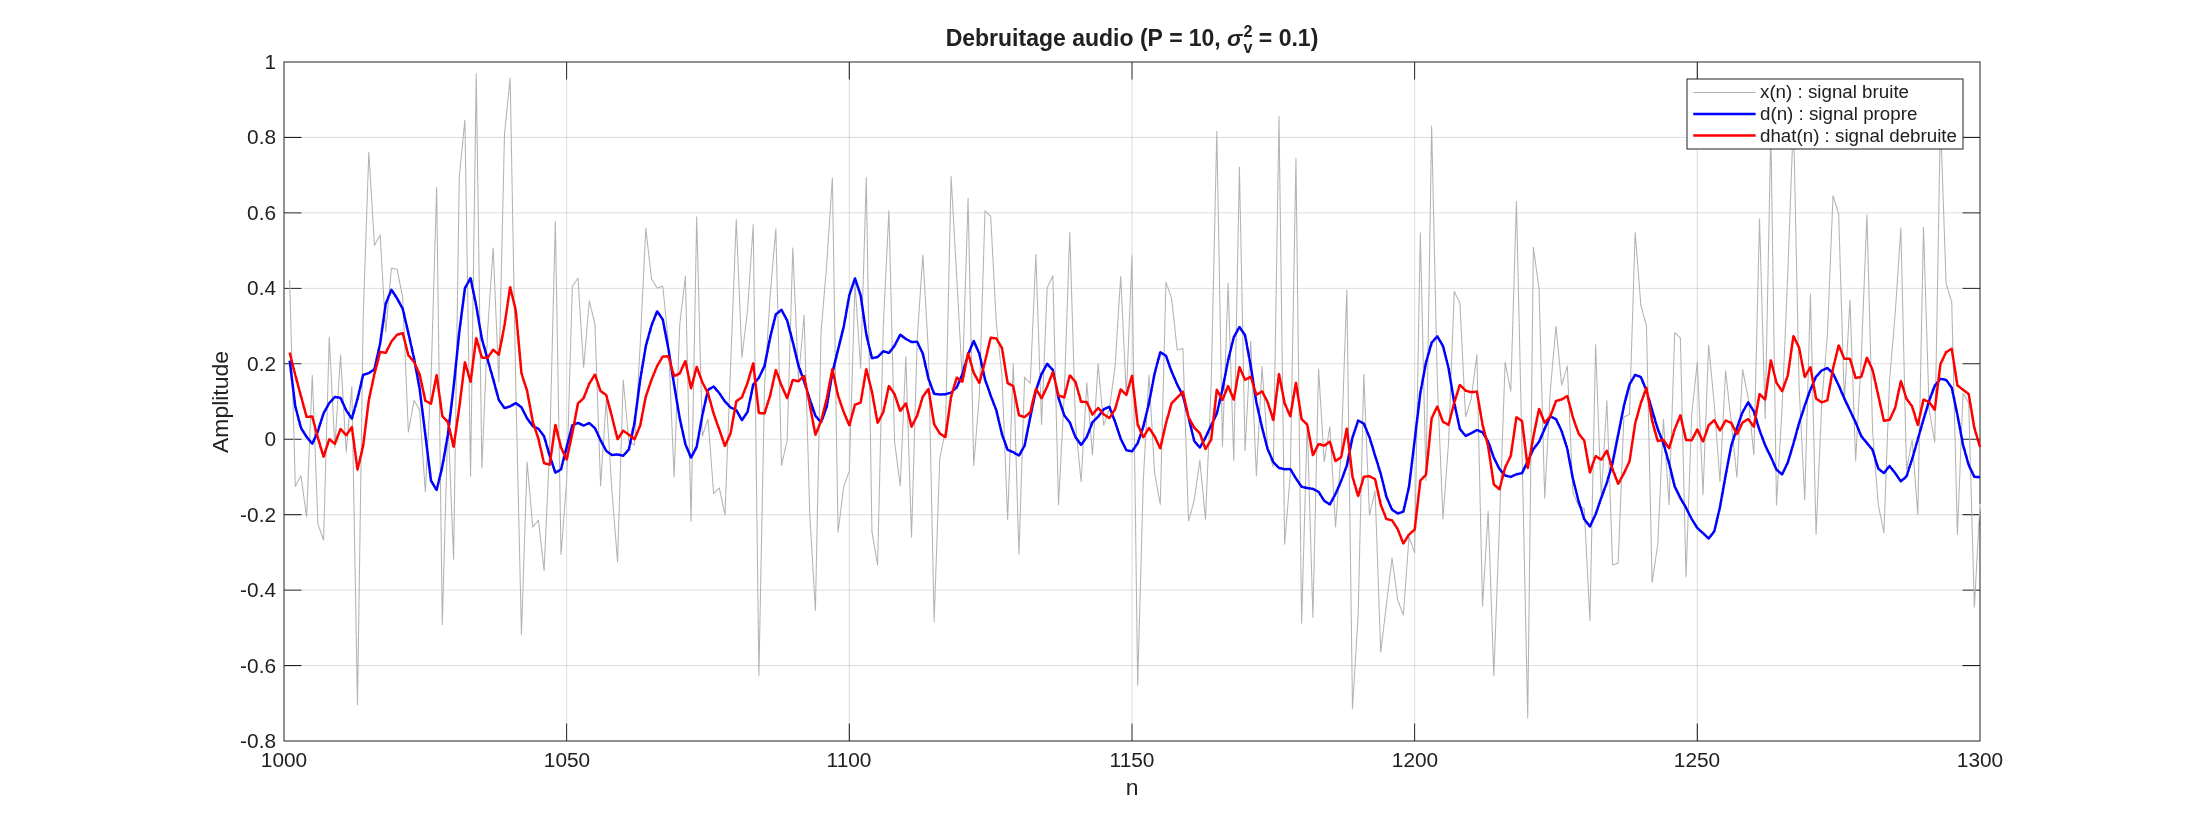
\includegraphics[width=\linewidth]{p3_qa_signaux}
  \caption{Signal bruité $x(n)$, signal propre $d(n)$ et signal débruité $\hat d(n)$ ($P=10$, $\sigma_v^2=0.1$).}
\end{figure}

\begin{resultat}
$\mathrm{EQM}_{\min}=0.0155$ ; $\mathrm{RSB}_{\mathrm{av}}\approx-3.9$~dB, $\mathrm{RSB}_{\mathrm{ap}}\approx 4.2$~dB, soit un gain d'environ $8.1$~dB.
\end{resultat}

\begin{interpretation}
\begin{itemize}
  \item \textbf{Performance.} L'erreur passe de $0.1$ (sans filtrage) à $0.0155$. Elle est aussi bien inférieure à celle d'une sortie nulle ($P_d=0.0411$) : le filtre récupère réellement une partie du signal.
  \item \textbf{Allure.} $\hat d(n)$ suit l'allure de $d(n)$ et est beaucoup plus lisse que $x(n)$, mais les pics sont atténués et légèrement retardés : le filtre est une moyenne pondérée des $P$ derniers échantillons.
  \item \textbf{Comparaison avec la partie~2.} Le gain est supérieur à celui de la sinusoïde pour $P=10$ ($5.4$~dB), mais le RSB de départ est très différent ($-3.9$~dB contre $7$~dB) : le gain augmente mécaniquement quand le bruit domine (voir (c), (d) et (f)).
  \item \textbf{Écoute.} Les vagues (basses fréquences) sont conservées, les chants d'oiseaux (aigus) sont atténués avec le bruit : le filtre se comporte en passe-bas.
\end{itemize}
\end{interpretation}

\subsection{Question (b) : reprise des questions (e) et (f) de la partie 2}

\begin{enonce}
\textbf{Énoncé :} Reprendre les questions (e) et (f) de la partie~2 : pour $\sigma_v^2=0.1$, tracer $\mathrm{EQM}_{\min}$ puis le gain en RSB en fonction de $P$ (de 5 à 50, pas de 5). Choisir le meilleur ordre $P$.
\end{enonce}

\textbf{Démarche.} Un seul signal bruité pour tous les $P$. Les corrélations sont estimées une fois jusqu'au retard $49$ ; pour chaque $P$ on garde les $P$ premiers retards et on calcule $\mathrm{EQM}_{\min}$ et $\mathrm{gain}|_{\mathrm{dB}}=10\log_{10}(\sigma_v^2/\mathrm{EQM}_{\min})$.

\textbf{Code.}
\begin{lstlisting}
clear; clc; close all;
rng(0);

% Signal (comme en (a))
[y, Fs] = audioread('monson.wav');
y = y(:,1);
N = 1e5;  debut = round(1*Fs);
d = y(debut+1 : debut+N);
d = d / max(abs(d));

sigv2 = 0.1;
x = d + sqrt(sigv2)*randn(N,1);      % meme bruit pour tous les P

Plist  = 5:5:50;
EQMmin = zeros(size(Plist));
gain   = zeros(size(Plist));

% Correlations calculees une seule fois jusqu'au retard max
Pmax = max(Plist);
rxF = xcorr(x, Pmax-1, 'biased'); rxF = rxF(Pmax:end);
rdF = xcorr(d, Pmax-1, 'biased'); rdF = rdF(Pmax:end);

RSB_av = 10*log10(rdF(1)/sigv2);

for m = 1:length(Plist)
    P  = Plist(m);
    rx = rxF(1:P);  rd = rdF(1:P);   % P premiers retards
    wopt = toeplitz(rx) \ rd;
    EQMmin(m) = rd(1) - wopt'*rd;
    gain(m)   = 10*log10(rd(1)/EQMmin(m)) - RSB_av;
    fprintf('P = %2d : EQM_min = %.5f | gain = %.2f dB\n', ...
            P, EQMmin(m), gain(m));
end

% EQM_min en fonction de P
figure;
plot(Plist, EQMmin, 'bo-', 'LineWidth', 1.3); grid on;
xlabel('P'); ylabel('EQM_{min}');
saveas(gcf, 'figs_partie3/p3_qb_eqm.png');

% Gain en fonction de P
figure;
plot(Plist, gain, 'ro-', 'LineWidth', 1.3); grid on;
xlabel('P'); ylabel('gain (dB)');
saveas(gcf, 'figs_partie3/p3_qb_gain.png');
\end{lstlisting}

\begin{figure}[H]
  \centering
  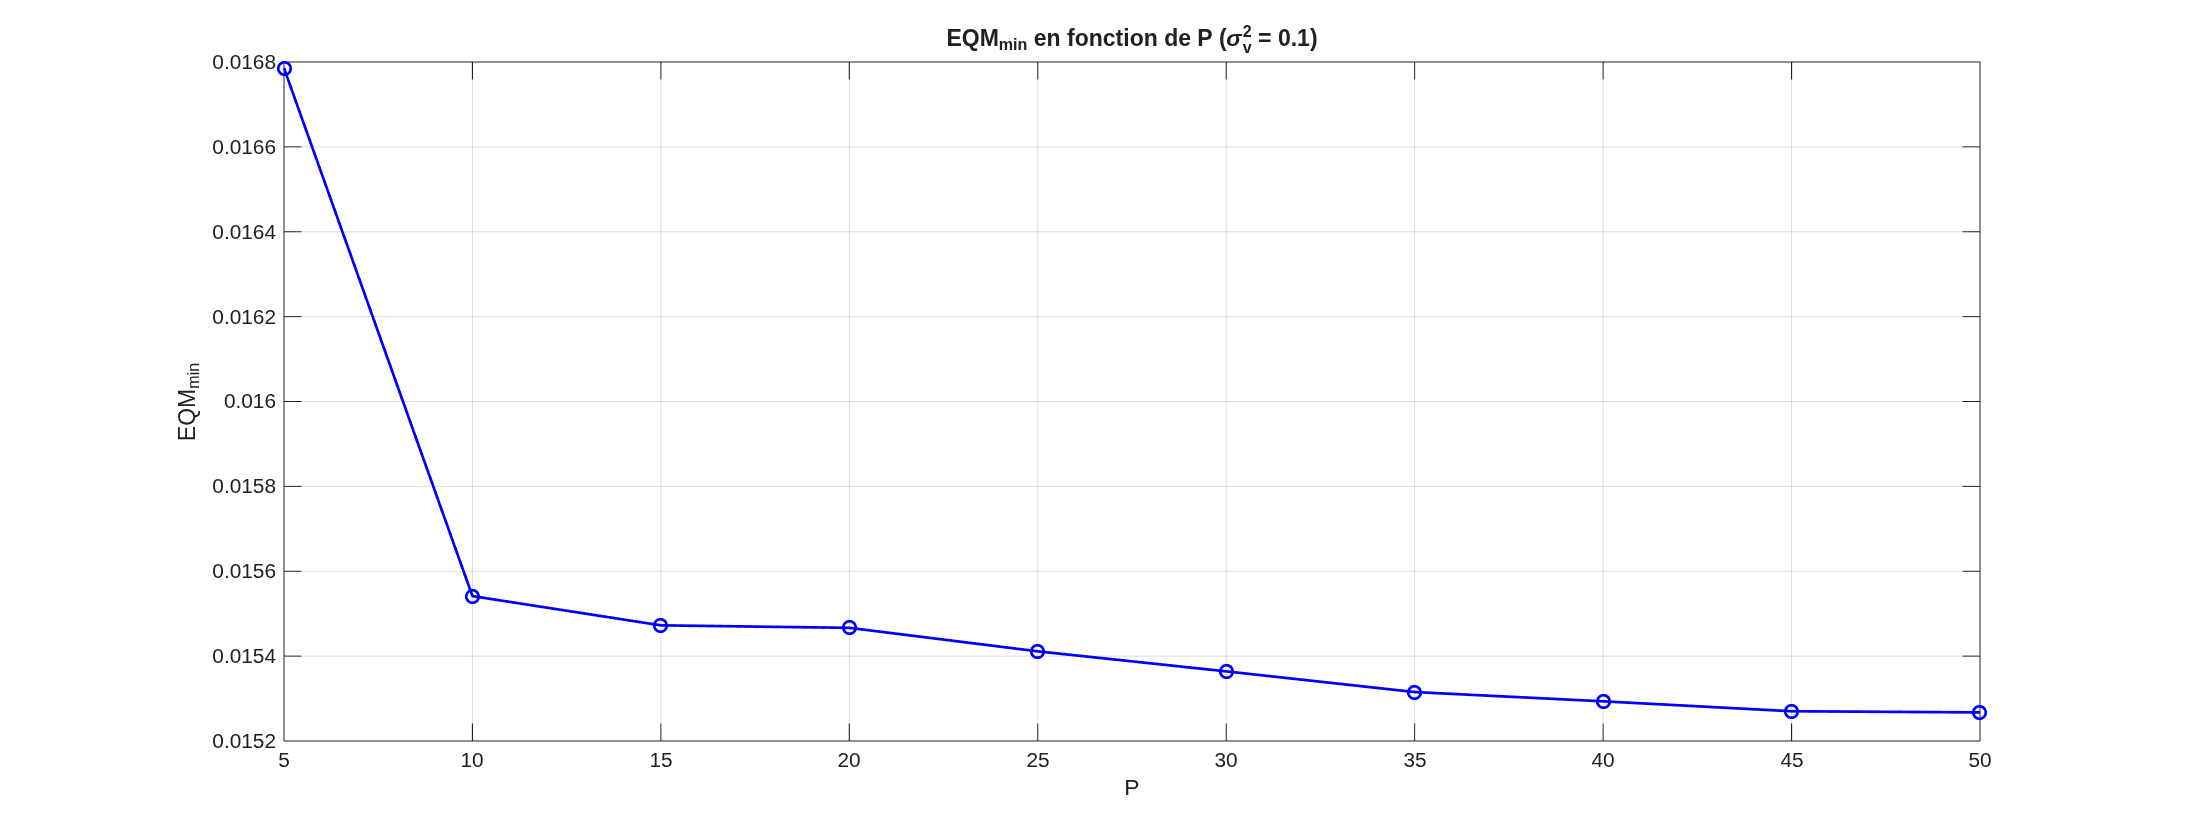
\includegraphics[width=\linewidth]{p3_qb_eqm}
  \caption{$\mathrm{EQM}_{\min}$ en fonction de $P$ ($\sigma_v^2=0.1$, signal audio).}
\end{figure}

\begin{figure}[H]
  \centering
  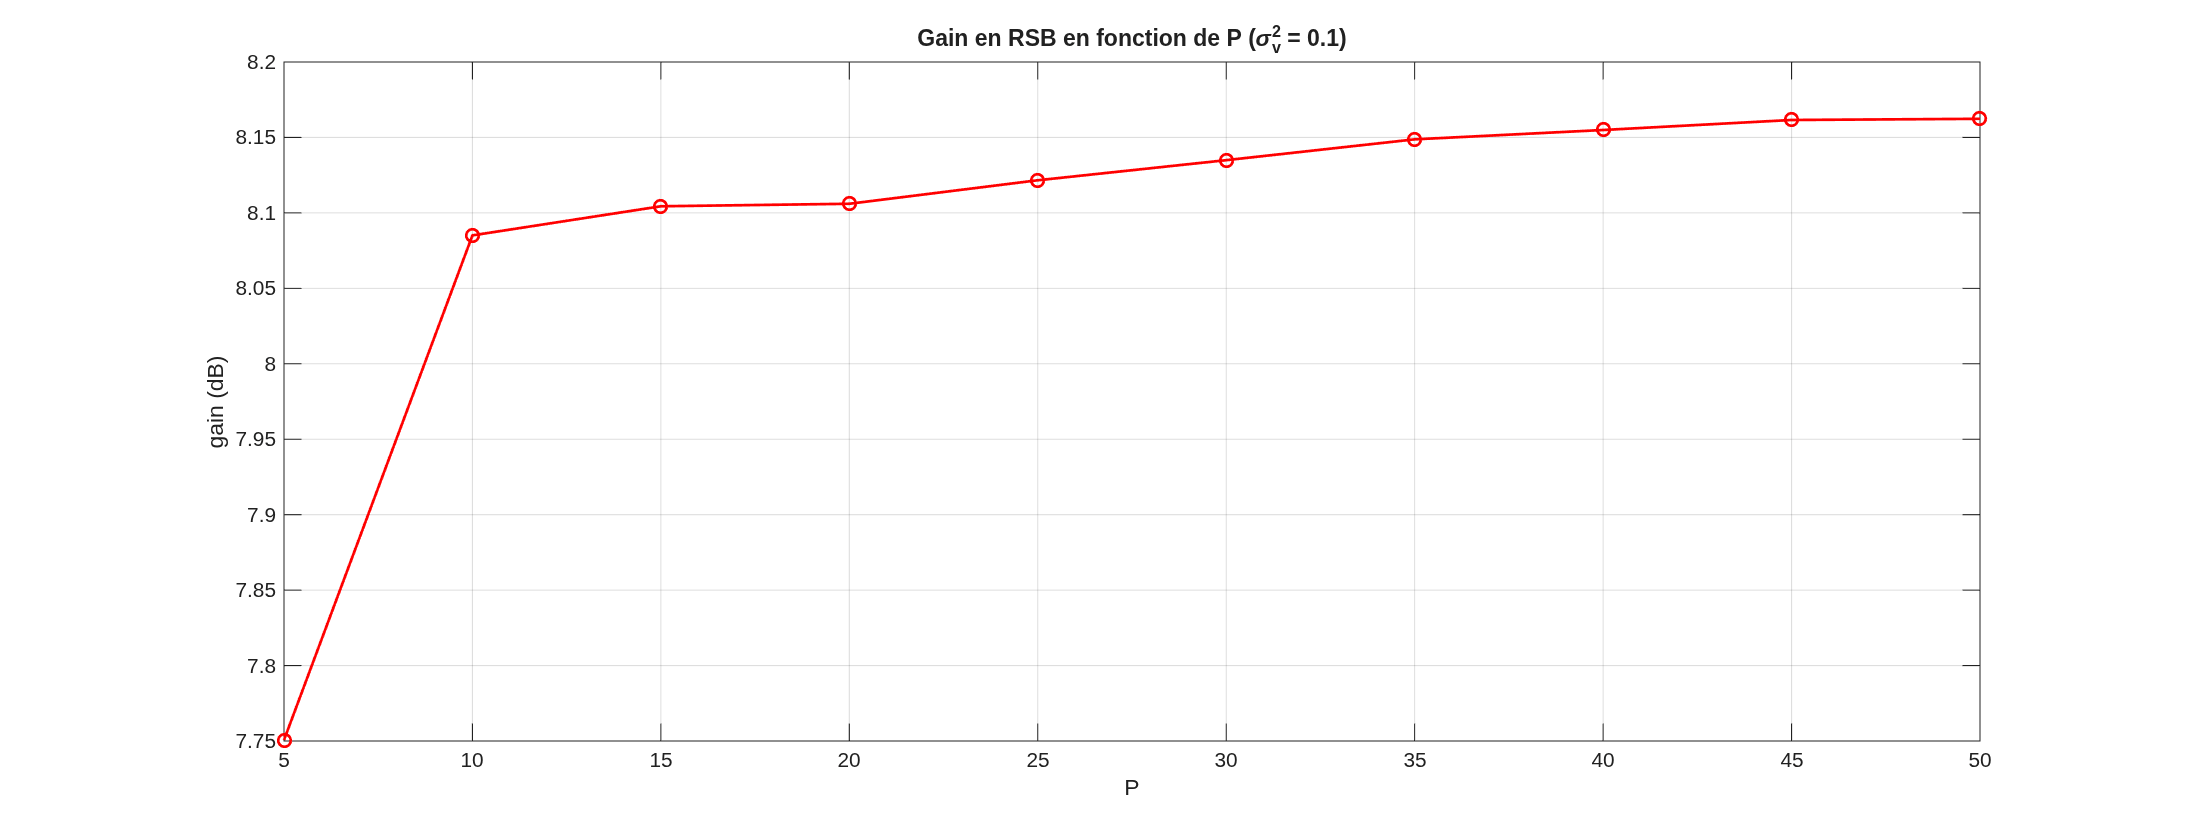
\includegraphics[width=\linewidth]{p3_qb_gain}
  \caption{Gain en RSB en fonction de $P$ ($\sigma_v^2=0.1$, signal audio).}
\end{figure}

\begin{interpretation}
\begin{itemize}
  \item \textbf{Évolution.} $\mathrm{EQM}_{\min}$ passe de $0.0168$ ($P=5$) à $0.0155$ ($P=10$), puis à $0.0153$ ($P=50$). Le gain passe de $7.75$ à $8.09$~dB, puis ne gagne que $0.08$~dB jusqu'à $P=50$. Attention à l'échelle zoomée : le gain ne varie que de $0.4$~dB sur toute la plage. Pour $P=10$, on retrouve le gain de (a) (même bruit grâce à \texttt{rng(0)}).
  \item \textbf{Explication.} La corrélation du signal audio décroît vite : les échantillons éloignés n'apportent presque plus d'information. À $F_s=44100$~Hz, 10 échantillons ($\approx 0.23$~ms) suffisent à exploiter l'essentiel de cette corrélation. Pour la sinusoïde, dont la corrélation ne décroît pas, le palier n'était atteint que vers $P=25$.
\end{itemize}
\end{interpretation}

\begin{resultat}[Meilleur choix de l'ordre]
$P=10$ : c'est le coude des courbes, le plus petit ordre donnant presque le gain maximal. Un ordre plus grand augmente le coût de calcul pour un gain négligeable.
\end{resultat}

\subsection{Question (c) : débruitage par trames de 3 ms}

\begin{enonce}
\textbf{Énoncé :} Réaliser le débruitage par trames de 3~ms : sur chaque trame $i$, filtre de Wiener $\mathbf{w}^i_{opt}=(\mathbf{R}^i_x)^{-1}\mathbf{r}^i_{d}$, où $\mathbf{R}^i_x$ est la matrice d'autocorrélation de la trame $i$ du signal bruité et $\mathbf{r}^i_{d}$ le vecteur d'autocorrélation de la trame $i$ du signal de référence, pour $P=10$ et $\sigma_v^2=0.5$. Donner le code (fonction \texttt{debruitage\_sig}), afficher $\mathrm{gain}|_{\mathrm{dB}}$ en fonction du numéro de trame $i$ et le comparer au gain obtenu sur tout le signal. Donner la ou les lignes de code permettant de reconstruire le signal à partir des trames débruitées.
\end{enonce}

\textbf{Démarche.}
\begin{enumerate}
  \item \textbf{Découpage.} $L=\mathrm{round}(3\cdot10^{-3}F_s)=132$ échantillons par trame, soit $K=\lfloor N/L\rfloor=757$ trames (les $76$ derniers échantillons sont ignorés).
  \item \textbf{Fonction \texttt{debruitage\_sig(d, P, sigv2)}} : bruite la trame, estime $r_x(k)$ et $r_d(k)$ sur la trame seule, calcule $\mathbf{w}_{opt}$, filtre, et renvoie $x$, $\hat d$, $\mathrm{gain}|_{\mathrm{dB}}=10\log_{10}(P_v/P_e)$ et $\mathrm{EQM}_{\min}$.
  \item \textbf{Débruitage par trames} : appel sur chaque trame et replacement des trames débruitées à leur position.
  \item \textbf{Référence} : même fonction appliquée à tout le signal (un seul filtre).
\end{enumerate}

\textbf{Code.} Fonction de débruitage (\texttt{debruitage\_sig.m}) :
\begin{lstlisting}
function [x, dhat, gain_dB, EQMmin] = debruitage_sig(d, P, sigv2)
% Debruitage d'un signal d par filtre de Wiener d'ordre P
% Entrees : d (signal propre), P (ordre), sigv2 (variance du bruit)
% Sorties : x (signal bruite), dhat (signal debruite), gain en dB, EQM_min
d = d(:);
N = length(d);
v = sqrt(sigv2)*randn(N,1);          % bruit blanc gaussien
x = d + v;                           % signal bruite

rx = xcorr(x, P-1, 'biased'); rx = rx(P:end);
rd = xcorr(d, P-1, 'biased'); rd = rd(P:end);
wopt = toeplitz(rx) \ rd;            % filtre de Wiener
dhat = filter(wopt, 1, x);           % signal debruite
EQMmin = rd(1) - wopt'*rd;           % EQM minimale (formule)

% Gain mesure : erreur avant (bruit) / erreur apres (residu)
Pd     = rd(1);
RSB_av = 10*log10(Pd / mean(v.^2));
RSB_ap = 10*log10(Pd / mean((d - dhat).^2));
gain_dB = RSB_ap - RSB_av;
end
\end{lstlisting}

Script principal (\texttt{Question\_c.m}) :
\begin{lstlisting}
clear; clc; close all;
rng(0);

% Signal
[y, Fs] = audioread('monson.wav');
y = y(:,1);
N = 1e5;  debut = round(1*Fs);
d = y(debut+1 : debut+N);
d = d / max(abs(d));
P = 10;  sigv2 = 0.5;

% Decoupage en trames de 3 ms
L = round(3e-3 * Fs);                % 132 echantillons par trame
K = floor(N / L);                    % nombre de trames
fprintf('L = %d echantillons/trame | K = %d trames\n', L, K);

gains    = zeros(K,1);
EQMs     = zeros(K,1);
x_rec    = zeros(K*L,1);
dhat_rec = zeros(K*L,1);

% Debruitage trame par trame
for i = 1:K
    idx = (i-1)*L+1 : i*L;           % indices de la trame i
    [xi, dhi, gains(i), EQMs(i)] = debruitage_sig(d(idx), P, sigv2);
    x_rec(idx)    = xi;              % reconstruction du signal bruite
    dhat_rec(idx) = dhi;             % reconstruction du signal debruite
end

% Debruitage sur tout le signal (reference)
[x_g, dhat_g, gain_g, EQM_g] = debruitage_sig(d, P, sigv2);
fprintf('Gain global (tout le signal)  = %.2f dB\n', gain_g);
fprintf('Gain moyen par trame          = %.2f dB\n', mean(gains));

% Gain par trame
figure;
plot(1:K, gains, 'b.-'); hold on;
yline(gain_g, 'r--', 'LineWidth', 1.5);
yline(mean(gains), 'k:', 'LineWidth', 1.5);
grid on; xlabel('numero de trame i'); ylabel('gain (dB)');
legend('gain par trame', 'gain global', 'gain moyen par trame');
saveas(gcf, 'figs_partie3/p3_qc_gain_trames.png');

% Ecoute : debruitage global puis par trames
sound(dhat_g, Fs);    pause(N/Fs + 0.5);
sound(dhat_rec, Fs);
\end{lstlisting}

\begin{resultat}[Reconstruction du signal]
Chaque trame débruitée est replacée à sa position dans la boucle :
\begin{lstlisting}[numbers=none]
idx = (i-1)*L+1 : i*L;
dhat_rec(idx) = dhi;
\end{lstlisting}
\end{resultat}

\begin{figure}[H]
  \centering
  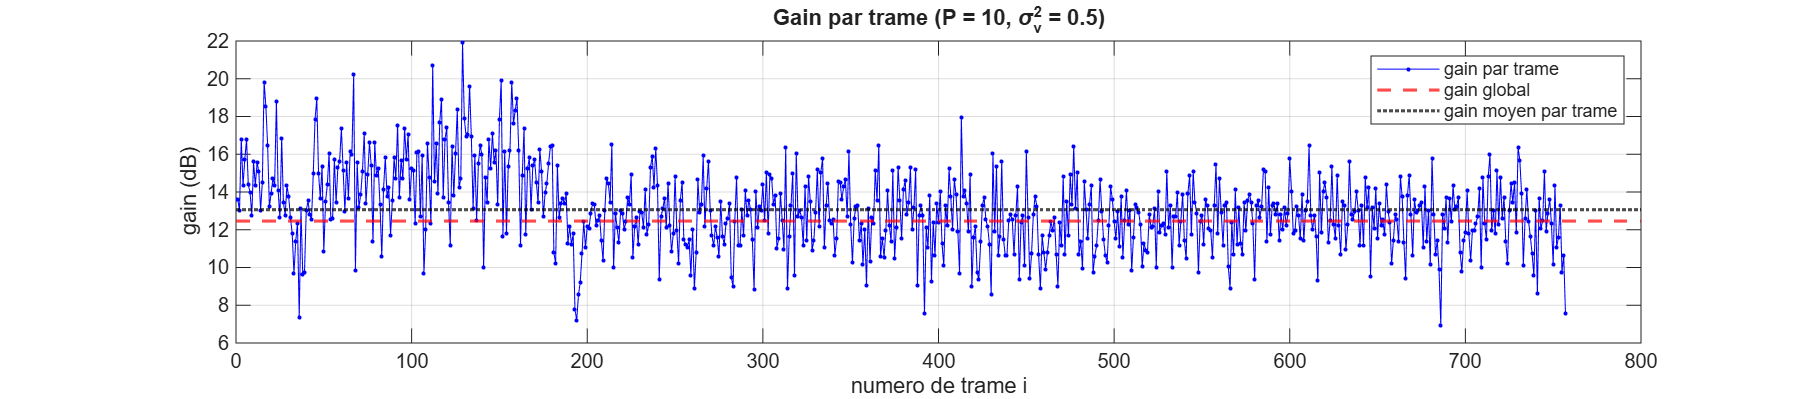
\includegraphics[width=\linewidth]{p3_qc_gain_trames}
  \caption{Gain en RSB de chaque trame de 3~ms, comparé au gain global et au gain moyen par trame ($P=10$, $\sigma_v^2=0.5$).}
\end{figure}

\begin{resultat}
$K=757$ trames de $L=132$ échantillons. Gain global : $12.46$~dB ; gain moyen par trame : $13.06$~dB (+0.6~dB).
\end{resultat}

\begin{interpretation}
\begin{itemize}
  \item \textbf{Comparaison.} Le gain moyen par trame dépasse le gain global : le signal audio n'est pas stationnaire (vagues, chants d'oiseaux), un filtre par trame s'adapte aux statistiques locales, alors qu'un filtre unique est un compromis moyen. Sur 3~ms, le signal est à peu près stationnaire, ce qui justifie le filtre de Wiener.
  \item \textbf{Dispersion.} La plupart des trames sont entre $10$ et $16$~dB, avec des chutes vers $7$~dB (trames $\approx 40$, $200$, $690$) et des pics à $20$--$22$~dB parmi les $\approx 180$ premières trames. Causes : contenu variable d'une trame à l'autre (le gain dépend de la puissance de la trame, voir (d)), corrélations estimées sur seulement $132$ échantillons, et transitoire de $P-1=9$ échantillons ($7\,\%$ de la trame) car le filtre redémarre à zéro à chaque trame.
  \item \textbf{Nuances.} La moyenne de gains en dB n'est pas le gain du signal reconstruit (en (e), l'écart réel n'est que de $\approx 0.2$~dB) ; le traitement par trames coûte $757$ résolutions de systèmes au lieu d'une.
  \item \textbf{Gain global plus élevé qu'en (a)} ($12.46$ contre $8.1$~dB) : non pas parce que le signal est mieux reconstruit, mais parce que l'erreur reste bornée par $\approx P_d$ alors que $P_v$ augmente ; le gain croît donc mécaniquement avec le bruit.
\end{itemize}
\end{interpretation}

\subsection{Question (d) : étude statistique du gain et de \texorpdfstring{$\mathrm{EQM}_{\min}$}{EQMmin} par trame}

\begin{enonce}
\textbf{Énoncé :} Faire de même pour $\mathrm{EQM}_{\min}$ en comparant les résultats des différentes trames. Donner une description statistique des valeurs de $\mathrm{gain}|_{\mathrm{dB}}$ et $\mathrm{EQM}_{\min}$ et interpréter. Quelle fonction MATLAB peut-on utiliser pour décrire la distribution des valeurs ?
\end{enonce}

\textbf{Démarche.} Même découpage et même bruit qu'en (c). Pour chaque trame : $\mathrm{gain}|_{\mathrm{dB}}$, $\mathrm{EQM}^i_{\min}$ et la puissance $P^i_d$. Statistiques : moyenne, écart-type, médiane, min, max, quartiles $Q_1$ et $Q_3$ ; distributions tracées avec \texttt{histogram} ; gain tracé en fonction de $P^i_d$ pour expliquer la dispersion.

\textbf{Code.} (\texttt{debruitage\_sig.m} dans le même dossier)
\begin{lstlisting}
clear; clc; close all;
rng(0);                              % meme bruit qu'en (c)
figDir = 'figs_partie3';

% Signal (comme en (c))
[y, Fs] = audioread('monson.wav');
y = y(:,1);
N = 1e5;  debut = round(1*Fs);
d = y(debut+1 : debut+N);
d = d / max(abs(d));
P = 10;  sigv2 = 0.5;

% Decoupage en trames de 3 ms
L = round(3e-3 * Fs);
K = floor(N / L);

gains = zeros(K,1);
EQMs  = zeros(K,1);
Pds   = zeros(K,1);                  % puissance de chaque trame

% Debruitage trame par trame
for i = 1:K
    idx = (i-1)*L+1 : i*L;
    [~, ~, gains(i), EQMs(i)] = debruitage_sig(d(idx), P, sigv2);
    S = 0;
    for k = idx
        S = S + d(k)^2;
    end
    Pds(i) = S / L;
end

% Debruitage sur tout le signal (reference)
[~, ~, gain_g, EQM_g] = debruitage_sig(d, P, sigv2);

% Description statistique
gs = sort(gains);  es = sort(EQMs);
fprintf('Gain : moy = %.2f | std = %.2f | med = %.2f\n', ...
        mean(gains), std(gains), median(gains));
fprintf('min = %.2f | max = %.2f | Q1 = %.2f | Q3 = %.2f | global = %.2f\n', ...
        gs(1), gs(end), gs(round(0.25*K)), gs(round(0.75*K)), gain_g);
fprintf('EQM : moy = %.4f | std = %.4f | med = %.4f\n', ...
        mean(EQMs), std(EQMs), median(EQMs));
fprintf('min = %.4f | max = %.4f | Q1 = %.4f | Q3 = %.4f | global = %.4f\n', ...
        es(1), es(end), es(round(0.25*K)), es(round(0.75*K)), EQM_g);
fprintf('Trames avec EQM_min < 0 : %d\n', sum(EQMs < 0));

% EQM_min par trame
figure;
plot(1:K, EQMs, 'b.-'); hold on;
yline(EQM_g, 'r--', 'LineWidth', 1.5);
yline(mean(EQMs), 'k:', 'LineWidth', 1.5);
grid on; xlabel('numero de trame i'); ylabel('EQM_{min}');
legend('EQM_{min} par trame', 'EQM_{min} global', 'EQM_{min} moyenne', ...
       'Location', 'best');
saveas(gcf, fullfile(figDir, 'p3_qd_eqm_trames.png'));

% Histogramme du gain
figure;
histogram(gains, 30); hold on;
xline(gain_g, 'r--', 'LineWidth', 1.5);
xline(mean(gains), 'k:', 'LineWidth', 1.5);
grid on; xlabel('gain (dB)'); ylabel('nombre de trames');
legend('trames', 'gain global', 'gain moyen', 'Location', 'best');
saveas(gcf, fullfile(figDir, 'p3_qd_hist_gain.png'));

% Histogramme de EQM_min
figure;
histogram(EQMs, 30); hold on;
xline(EQM_g, 'r--', 'LineWidth', 1.5);
xline(mean(EQMs), 'k:', 'LineWidth', 1.5);
grid on; xlabel('EQM_{min}'); ylabel('nombre de trames');
legend('trames', 'EQM_{min} global', 'EQM_{min} moyenne', 'Location', 'best');
saveas(gcf, fullfile(figDir, 'p3_qd_hist_eqm.png'));

% Gain en fonction de la puissance de la trame
figure;
plot(Pds, gains, 'b.'); grid on;
xlabel('puissance de la trame P_d^i'); ylabel('gain (dB)');
saveas(gcf, fullfile(figDir, 'p3_qd_gain_vs_puissance.png'));
\end{lstlisting}

\begin{figure}[H]
  \centering
  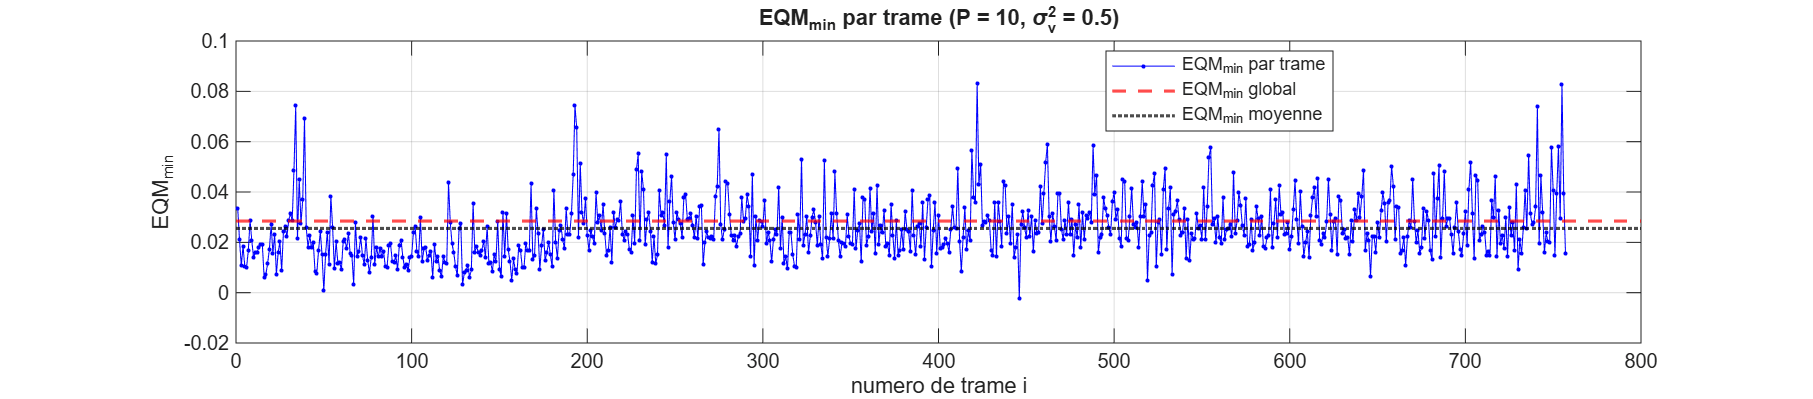
\includegraphics[width=\linewidth]{p3_qd_eqm_trames}
  \caption{$\mathrm{EQM}_{\min}$ de chaque trame, comparée à $\mathrm{EQM}_{\min}$ globale et à la moyenne des trames ($P=10$, $\sigma_v^2=0.5$).}
\end{figure}

\begin{figure}[H]
  \centering
  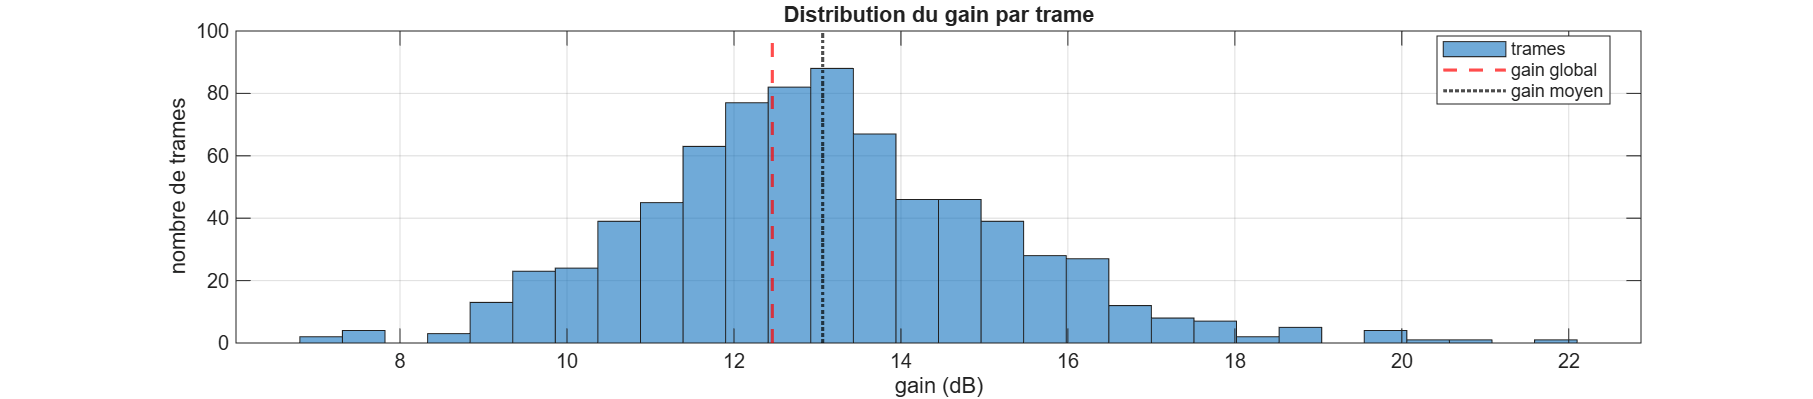
\includegraphics[width=\linewidth]{p3_qd_hist_gain}

  \medskip
  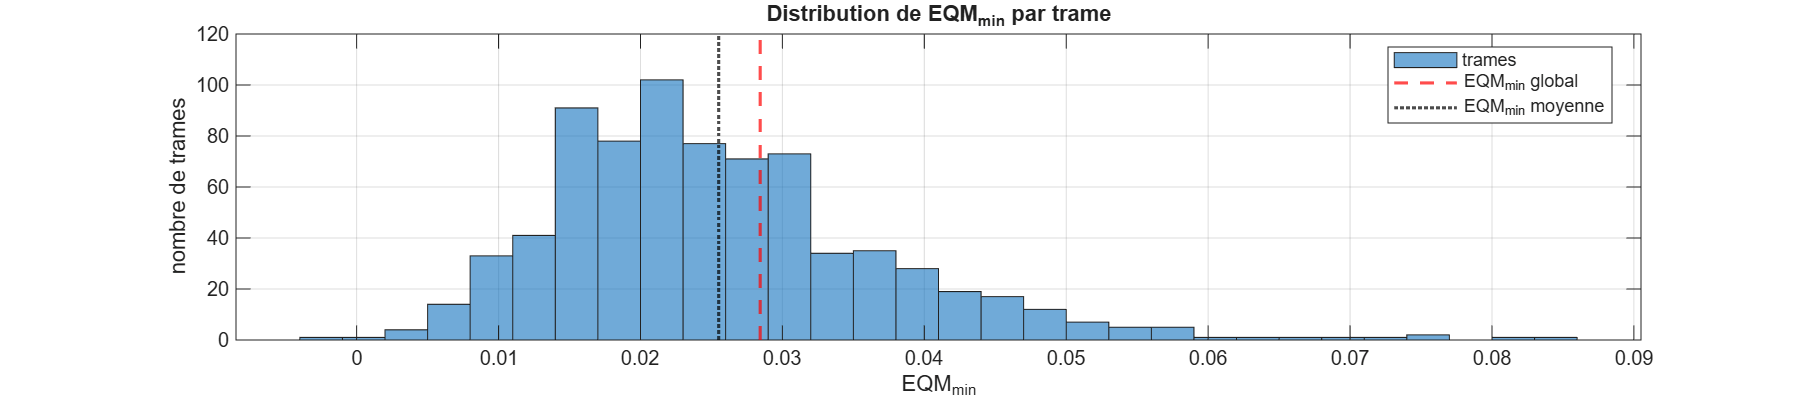
\includegraphics[width=\linewidth]{p3_qd_hist_eqm}
  \caption{Distributions du gain (en haut) et de $\mathrm{EQM}_{\min}$ (en bas) sur les $757$ trames (fonction \texttt{histogram}).}
\end{figure}

\begin{figure}[H]
  \centering
  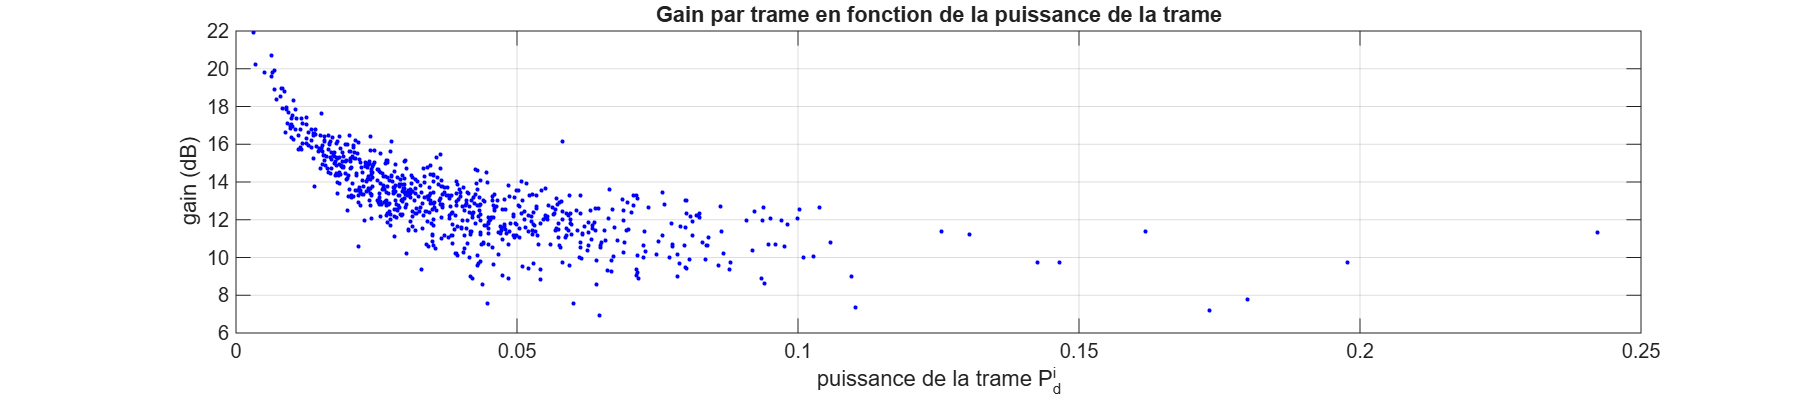
\includegraphics[width=\linewidth]{p3_qd_gain_vs_puissance}
  \caption{Gain de chaque trame en fonction de sa puissance $P^i_d$.}
\end{figure}

\begin{table}[H]
  \centering
  \begin{tabular}{lccccccc}
    \toprule
     & Moyenne & Écart-type & Médiane & Min & Max & $Q_1$ & $Q_3$ \\
    \midrule
    $\mathrm{gain}|_{\mathrm{dB}}$ (dB) & 13.06 & 2.14 & 12.94 & 6.92 & 21.90 & 11.66 & 14.34 \\
    $\mathrm{EQM}_{\min}$ & 0.0255 & 0.0118 & 0.0234 & $-0.0025$ & 0.0832 & 0.0171 & 0.0313 \\
    \bottomrule
  \end{tabular}
  \caption{Description statistique sur les $757$ trames. Sur tout le signal : $\mathrm{gain}|_{\mathrm{dB}}=12.46$~dB et $\mathrm{EQM}_{\min}=0.0284$.}
\end{table}

\begin{resultat}[Fonction MATLAB]
\texttt{histogram} (ou \texttt{hist}) pour la distribution, complétée par \texttt{mean}, \texttt{std}, \texttt{median}, \texttt{min}, \texttt{max} ; \texttt{boxplot} (Statistics Toolbox) résume médiane, quartiles et valeurs extrêmes en une figure.
\end{resultat}

\begin{interpretation}
\begin{itemize}
  \item \textbf{Comparaison au global.} $\mathrm{EQM}_{\min}$ moyenne des trames : $0.0255$, contre $0.0284$ sur tout le signal. Cohérent avec le gain moyen plus élevé trouvé en (c).
  \item \textbf{Distribution du gain.} En cloche, quasi symétrique : moyenne ($13.06$) $\approx$ médiane ($12.94$~dB). La moitié des trames est entre $11.66$ et $14.34$~dB, mais l'étendue est large ($6.92$ à $21.90$~dB), avec une petite queue vers les forts gains.
  \item \textbf{Distribution de $\mathrm{EQM}_{\min}$.} Dissymétrique, avec une queue vers les grandes valeurs (jusqu'à $0.083$) : moyenne $>$ médiane. Dispersion forte (écart-type $\approx$ moitié de la moyenne). Les $\approx 180$ premières trames ont une erreur plus faible ($0.01$--$0.02$).
  \item \textbf{Valeur négative.} Une trame donne $\mathrm{EQM}_{\min}=-0.0025$, physiquement impossible : c'est l'erreur d'estimation de la partie~2 ($r_{dx}=r_d$ supposé), fortement amplifiée par l'estimation sur $132$ échantillons.
  \item \textbf{Origine de la dispersion du gain.} Plus la trame est faible, plus le gain est élevé : $17$--$22$~dB pour $P^i_d<0.01$, $7$--$13$~dB pour $P^i_d>0.05$. Comme $\mathrm{gain}|_{\mathrm{dB}}=10\log_{10}(P_v/P_e)$ et que $P_e$ reste de l'ordre de $P^i_d$ au plus (le filtre atténue sa sortie quand le bruit domine), un fort gain signifie surtout que le bruit a été supprimé, pas que le signal est bien reconstruit. Les premières trames correspondent à un passage plus calme.
\end{itemize}
\end{interpretation}

\subsection{Question (e) : autocorrélation de référence calculée sur la trame 1}

\begin{enonce}
\textbf{Énoncé :} En supposant que l'autocorrélation du signal de référence a été calculée uniquement sur la trame n°1, réaliser le débruitage avec $\mathbf{w}^i_{opt}=(\mathbf{R}^i_x)^{-1}\mathbf{r}^1_{d}$. Comparer les performances par rapport aux deux démarches précédentes. Interpréter.
\end{enonce}

\textbf{Démarche.}
\begin{enumerate}
  \item Même découpage qu'en (c) ($K=757$, $L=132$, $P=10$, $\sigma_v^2=0.5$).
  \item Comparaison équitable : le bruit est généré \textbf{une seule fois}, les trois méthodes débruitent le même $x(n)$.
  \item $\mathbf{r}^1_{d}$ est calculé une fois sur la trame 1 ; pour chaque trame on estime $\mathbf{R}^i_x$ et on calcule les deux filtres $(\mathbf{R}^i_x)^{-1}\mathbf{r}^i_{d}$ (méthode (c)) et $(\mathbf{R}^i_x)^{-1}\mathbf{r}^1_{d}$ (méthode (e)).
  \item Chaque trame est filtrée avec ses $P-1$ échantillons précédents (pas de redémarrage à zéro).
  \item Critères : gain de chaque trame et gain $10\log_{10}(P_v/P_e)$ du signal \textbf{reconstruit}, plus fiable que la moyenne de gains en dB.
\end{enumerate}

\textbf{Code.}
\begin{lstlisting}
clear; clc; close all;
rng(0);
figDir = 'figs_partie3';

% Signal
[y, Fs] = audioread('monson.wav');
y = y(:,1);
N = 1e5;  debut = round(1*Fs);
d = y(debut+1 : debut+N);
d = d / max(abs(d));
P = 10;  sigv2 = 0.5;

% Decoupage en trames de 3 ms
L = round(3e-3 * Fs);
K = floor(N / L);
M = K*L;                             % echantillons couverts par les trames

% Bruit genere une seule fois : meme signal bruite pour les 3 methodes
v = sqrt(sigv2)*randn(N,1);
x = d + v;

% r_d calcule uniquement sur la trame 1
rd1 = xcorr(d(1:L), P-1, 'biased'); rd1 = rd1(P:end);

gain_i = zeros(K,1);                 % methode (c) : r_d de la trame i
gain_1 = zeros(K,1);                 % methode (e) : r_d de la trame 1
dhat_i = zeros(M,1);
dhat_1 = zeros(M,1);

for i = 1:K
    idx = (i-1)*L+1 : i*L;
    xi = x(idx);  di = d(idx);  vi = v(idx);

    % R_x et r_d de la trame i
    rx = xcorr(xi, P-1, 'biased'); rx = rx(P:end);
    Rx = toeplitz(rx);
    rdi = xcorr(di, P-1, 'biased'); rdi = rdi(P:end);

    % Les deux filtres
    h_i = Rx \ rdi;
    h_1 = Rx \ rd1;
    % Filtrage avec les P-1 echantillons precedents
    deb = max(1, idx(1) - (P-1));
    xe  = x(deb : idx(end));
    dh_i = filter(h_i, 1, xe);  dh_i = dh_i(end-L+1:end);
    dh_1 = filter(h_1, 1, xe);  dh_1 = dh_1(end-L+1:end);

    % Reconstruction
    dhat_i(idx) = dh_i;
    dhat_1(idx) = dh_1;

    % Gains de la trame
    Sv = 0; Se_i = 0; Se_1 = 0;
    for k = 1:L
        Sv   = Sv   + vi(k)^2;
        Se_i = Se_i + (di(k) - dh_i(k))^2;
        Se_1 = Se_1 + (di(k) - dh_1(k))^2;
    end
    gain_i(i) = 10*log10(Sv / Se_i);
    gain_1(i) = 10*log10(Sv / Se_1);
end

% Methode globale (un seul filtre pour tout le signal)
rx = xcorr(x, P-1, 'biased'); rx = rx(P:end);
rd = xcorr(d, P-1, 'biased'); rd = rd(P:end);
h_g = toeplitz(rx) \ rd;
dhat_g = filter(h_g, 1, x);

% Gain de chaque signal reconstruit
Sv = 0; Se_g = 0; Se_i = 0; Se_1 = 0;
for k = 1:M
    Sv   = Sv   + v(k)^2;
    Se_g = Se_g + (d(k) - dhat_g(k))^2;
    Se_i = Se_i + (d(k) - dhat_i(k))^2;
    Se_1 = Se_1 + (d(k) - dhat_1(k))^2;
end
G_g = 10*log10(Sv / Se_g);
G_i = 10*log10(Sv / Se_i);
G_1 = 10*log10(Sv / Se_1);

fprintf('global = %.2f | trames r_d^i = %.2f | trames r_d^1 = %.2f\n', ...
        G_g, G_i, G_1);
fprintf('r_d^i : moy = %.2f | med = %.2f | std = %.2f\n', ...
        mean(gain_i), median(gain_i), std(gain_i));
fprintf('r_d^1 : moy = %.2f | med = %.2f | std = %.2f\n', ...
        mean(gain_1), median(gain_1), std(gain_1));
fprintf('Trames ou r_d^1 fait mieux : %d / %d\n', sum(gain_1 > gain_i), K);

% Gain par trame avec r_d^1
figure;
plot(1:K, gain_1, 'm.-'); hold on;
yline(mean(gain_1), 'k:', 'LineWidth', 1.5);
yline(G_g, 'r--', 'LineWidth', 1.5);
grid on; xlabel('numero de trame i'); ylabel('gain (dB)');
legend('gain par trame (r_d^1)', 'gain moyen par trame', 'gain global', ...
       'Location', 'best');
drawnow;
exportgraphics(gcf, fullfile(figDir, 'p3_qe_gain_trames.png'), 'Resolution', 150);

% Comparaison des deux methodes par trame
figure;
plot(1:K, gain_i, 'b.-'); hold on;
plot(1:K, gain_1, 'm.-');
yline(G_g, 'r--', 'LineWidth', 1.5);
grid on; xlabel('numero de trame i'); ylabel('gain (dB)');
legend('r_d^i (question c)', 'r_d^1 (question e)', 'gain global', ...
       'Location', 'best');
drawnow;
exportgraphics(gcf, fullfile(figDir, 'p3_qe_comparaison.png'), 'Resolution', 150);

% Distributions des deux methodes
figure;
histogram(gain_i, 30, 'DisplayStyle', 'stairs', 'EdgeColor', 'b', 'LineWidth', 1.5); hold on;
histogram(gain_1, 30, 'DisplayStyle', 'stairs', 'EdgeColor', 'm', 'LineWidth', 1.5);
xline(G_g, 'r--', 'LineWidth', 1.5);
grid on; xlabel('gain (dB)'); ylabel('nombre de trames');
legend('r_d^i (question c)', 'r_d^1 (question e)', 'gain global', ...
       'Location', 'best');
drawnow;
exportgraphics(gcf, fullfile(figDir, 'p3_qe_hist.png'), 'Resolution', 150);

%% Ecoute (meme volume pour les trois)
soundsc(dhat_g, Fs);  pause(N/Fs + 0.5);
soundsc(dhat_i, Fs);  pause(N/Fs + 0.5);
soundsc(dhat_1, Fs);
\end{lstlisting}

\begin{figure}[H]
  \centering
  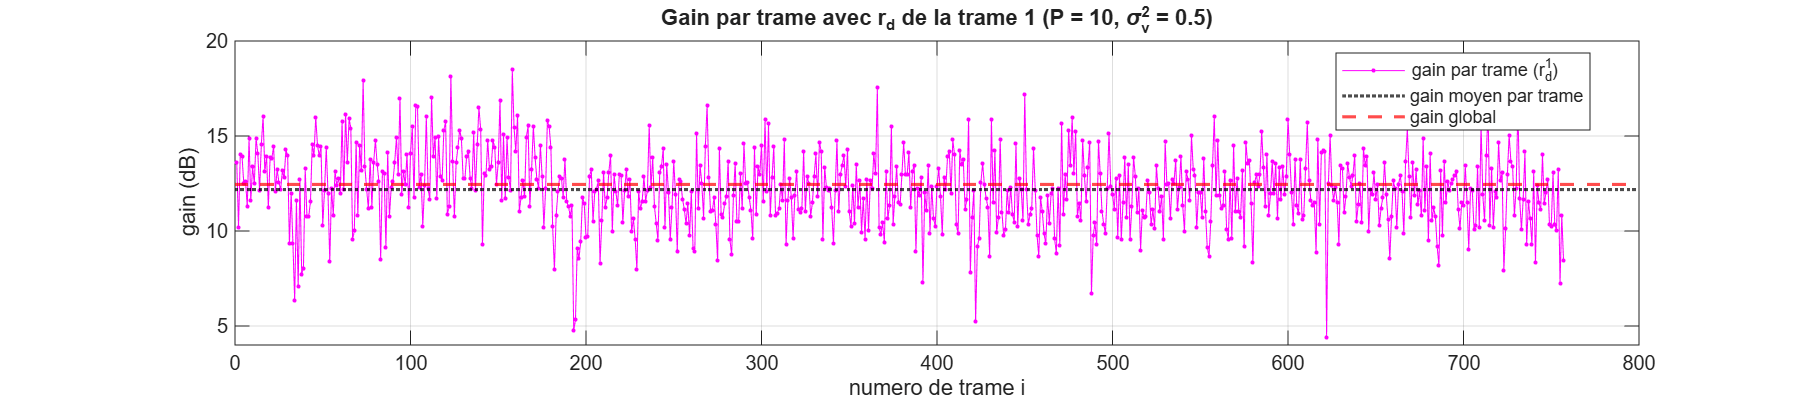
\includegraphics[width=\linewidth]{p3_qe_gain_trames}
  \caption{Gain par trame avec $\mathbf{r}^1_{d}$, comparé au gain moyen par trame et au gain global ($P=10$, $\sigma_v^2=0.5$).}
\end{figure}

\begin{figure}[H]
  \centering
  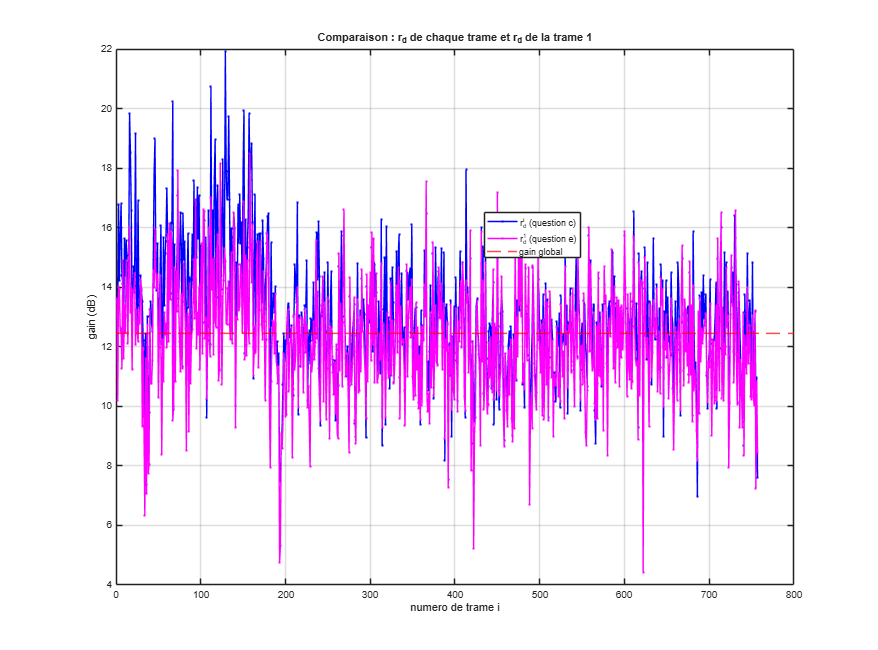
\includegraphics[width=0.85\linewidth]{p3_qe_comparaison}
  \caption{Gain par trame avec $\mathbf{r}^i_{d}$ (question c) et avec $\mathbf{r}^1_{d}$ (question e).}
\end{figure}

\begin{figure}[H]
  \centering
  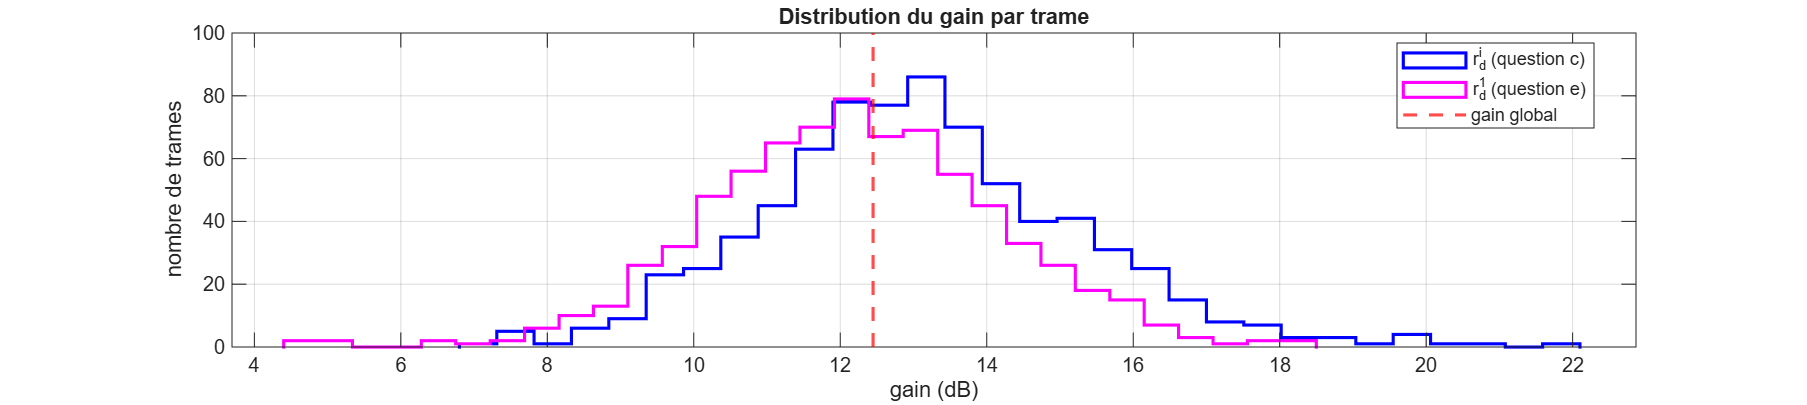
\includegraphics[width=\linewidth]{p3_qe_hist}
  \caption{Distribution du gain par trame pour les deux méthodes.}
\end{figure}

\begin{table}[H]
  \centering
  \begin{tabular}{lccc}
    \toprule
    Méthode & Filtre unique (global) & Trames, $\mathbf{r}^i_{d}$ (c) & Trames, $\mathbf{r}^1_{d}$ (e) \\
    \midrule
    Gain du signal reconstruit (dB) & 12.45 & 12.60 & 11.76 \\
    \bottomrule
  \end{tabular}
  \caption{Comparaison des trois démarches sur le même signal bruité ($P=10$, $\sigma_v^2=0.5$).}
\end{table}

\begin{resultat}
La méthode (e) est la moins bonne : $-0.8$~dB par rapport à (c) et $-0.7$~dB par rapport au filtre global. L'avantage réel de (c) sur le filtre global n'est que de $\approx 0.2$~dB (la moyenne des gains en dB annonçait $0.6$~dB).
\end{resultat}

\begin{interpretation}
\begin{itemize}
  \item \textbf{Par trame.} Avec $\mathbf{r}^1_{d}$, gain moyen $12.17$~dB et médiane $12.19$~dB (environ $13$~dB avec $\mathbf{r}^i_{d}$). Seules $166$ trames sur $757$ ($22\,\%$) font mieux qu'avec $\mathbf{r}^i_{d}$. L'histogramme est décalé d'environ $1$~dB vers la gauche : plus aucune trame au-delà de $18.5$~dB (contre $22$~dB), et des chutes jusqu'à $4.4$~dB (trames $\approx 35$, $193$, $420$, $622$). L'écart est surtout visible sur les $180$ premières trames.
  \item \textbf{Explication.} Utiliser $\mathbf{r}^1_{d}$ partout revient à supposer que le signal garde les statistiques de ses $3$ premières millisecondes : faux pour un signal non stationnaire. $\mathbf{R}^i_x$ et $\mathbf{r}^1_{d}$ décrivent alors deux portions différentes, et le filtre n'est plus optimal : il laisse passer trop de bruit si la trame $i$ est plus faible que la trame 1, et atténue trop si elle est plus forte. Le filtre global fait mieux car son autocorrélation est moyennée sur tout le signal, et non estimée sur $132$ échantillons.
  \item \textbf{Perte limitée} ($0.7$~dB) : $\mathbf{R}^i_x$ est toujours recalculée sur chaque trame, et les $10$ premiers retards de l'autocorrélation décrivent surtout le caractère passe-bas du signal, qui varie peu.
  \item \textbf{Intérêt pratique.} Ce cas est plus réaliste : on ne dispose en général du signal propre que sur une courte période d'apprentissage. Alternatives : estimer $r_d(k)=r_x(k)-\sigma_v^2\delta(k)$ à partir du signal bruité (testé en (f)), ou utiliser un filtre adaptatif LMS.
  \item \textbf{Écoute.} À volume égal, le débruitage global sonne mieux que les deux débruitages par trames, malgré un gain légèrement inférieur à (c) :
  \begin{itemize}
    \item \emph{clics toutes les 3~ms} dus au changement brusque des coefficients : saut moyen entre échantillons voisins de $0.065$ aux frontières contre $0.037$ ailleurs avec $\mathbf{r}^i_{d}$ ($0.069$ contre $0.044$ avec $\mathbf{r}^1_{d}$), contre $0.037$/$0.036$ pour le filtre global ; quelques filtres mal estimés produisent aussi des pics ($0.95$ contre $0.52$) ;
    \item \emph{plus de bruit résiduel} : $0.0104$ (et $0.0126$ avec $\mathbf{r}^1_{d}$) contre $0.0087$ pour le filtre global ; les trames réduisent l'EQM surtout en conservant plus de signal ($36\,\%$ contre $31\,\%$).
  \end{itemize}
  L'oreille étant plus sensible au bruit et aux clics qu'à une légère atténuation, le gain en RSB ne reflète pas la qualité perçue.
\end{itemize}
\end{interpretation}

\subsection{Question (f) : autres scénarios à étudier}

\begin{enonce}
\textbf{Énoncé :} Citer d'autres scénarios dont vous devez étudier les performances de ce type de débruitage.
\end{enonce}

\begin{resultat}[Scénarios à étudier]
\begin{enumerate}
  \item \textbf{Durée des trames} (compromis stationnarité / fiabilité des estimations / discontinuités) --- \emph{simulé ci-dessous}.
  \item \textbf{Signal propre indisponible} : $r_d(k)$ estimé à partir du signal bruité, $r_d(k)=r_x(k)-\sigma_v^2\delta(k)$ --- \emph{simulé}.
  \item \textbf{Niveau de bruit} (RSB d'entrée) --- \emph{simulé}.
  \item \textbf{Bruit coloré} (non blanc) --- \emph{simulé}.
  \item \textbf{Trames qui se chevauchent} avec fenêtre (Hann) et reconstruction par addition-recouvrement, pour supprimer les clics --- \emph{étudié en partie~4}.
  \item \textbf{$\sigma_v^2$ inconnue}, estimée sur un passage sans signal.
  \item \textbf{Bruit non stationnaire ou non gaussien} : impulsionnel, de puissance variable, bruit réel (rue, moteur, foule).
  \item \textbf{Autres signaux} : parole, musique, signaux biomédicaux.
  \item \textbf{Filtre adaptatif LMS} de Widrow, sans trames ni connaissance des statistiques.
  \item \textbf{Critères perceptifs} (PESQ, STOI) en complément du gain en RSB.
\end{enumerate}
\end{resultat}

\textbf{Démarche des simulations.} Même signal, $P=10$, \texttt{rng(0)}. Deux fonctions : \texttt{gain\_global} (un filtre sur tout le signal) et \texttt{gain\_trames} (un filtre par trame, avec les $P-1$ échantillons précédents). Les discontinuités sont mesurées par le rapport entre le saut moyen aux frontières des trames et le saut moyen sur tout le signal ($1$ = pas de discontinuité). Le bruit coloré est $v(n)=0.9\,v(n-1)+w(n)$, ramené à la même puissance que le bruit blanc.

\textbf{Code.}
\begin{lstlisting}
clear; clc; close all;
rng(0);
figDir = 'figs_partie3';

% Signal
[y, Fs] = audioread('monson.wav');
y = y(:,1);
N = 1e5;  debut = round(1*Fs);
d = y(debut+1 : debut+N);
d = d / max(abs(d));
P = 10;

%% Scenarios 1 et 2 : duree des trames et estimation de r_d
sigv2 = 0.5;
v = sqrt(sigv2)*randn(N,1);
x = d + v;

durees = [3 10 20 50 100];           % en ms
modes  = {'rdi', 'rd1', 'estime'};
nD = length(durees);  nM = length(modes);
G    = zeros(nD, nM);
saut = zeros(nD, nM);

G_glob = gain_global(d, x, v, P);
for k = 1:nD
    L = round(durees(k)*1e-3 * Fs);
    for m = 1:nM
        [G(k,m), saut(k,m)] = gain_trames(d, x, v, P, L, modes{m}, sigv2);
    end
    fprintf('trames %3d ms : r_d^i = %5.2f | r_d^1 = %5.2f | estime = %5.2f dB | global = %5.2f dB\n', ...
            durees(k), G(k,1), G(k,2), G(k,3), G_glob);
end
fprintf('saut frontieres / saut ailleurs (r_d^i) : %s\n', mat2str(saut(:,1)', 3));

% Gain en fonction de la duree des trames
figure;
plot(durees, G(:,1), 'b-o', 'LineWidth', 1.3); hold on;
plot(durees, G(:,2), 'm-s', 'LineWidth', 1.3);
plot(durees, G(:,3), 'g-^', 'LineWidth', 1.3);
yline(G_glob, 'r--', 'LineWidth', 1.5);
set(gca, 'XScale', 'log'); xticks(durees); grid on;
xlabel('duree des trames (ms)'); ylabel('gain du signal reconstruit (dB)');
legend('r_d^i (trame i)', 'r_d^1 (trame 1)', 'r_d estime depuis x', 'global', ...
       'Location', 'best');
drawnow;
exportgraphics(gcf, fullfile(figDir, 'p3_qf_gain_duree.png'), 'Resolution', 150);

% Discontinuites aux frontieres
figure;
plot(durees, saut(:,1), 'b-o', 'LineWidth', 1.3); hold on;
plot(durees, saut(:,2), 'm-s', 'LineWidth', 1.3);
plot(durees, saut(:,3), 'g-^', 'LineWidth', 1.3);
yline(1, 'k:', 'LineWidth', 1.5);
set(gca, 'XScale', 'log'); xticks(durees); grid on;
xlabel('duree des trames (ms)'); ylabel('saut frontieres / saut ailleurs');
legend('r_d^i (trame i)', 'r_d^1 (trame 1)', 'r_d estime depuis x', ...
       'sans discontinuite', 'Location', 'best');
drawnow;
exportgraphics(gcf, fullfile(figDir, 'p3_qf_saut_duree.png'), 'Resolution', 150);

%% Scenario 3a : niveau de bruit (trames de 20 ms)
sigList = [0.05 0.1 0.5 1];
nS  = length(sigList);
L20 = round(20e-3 * Fs);
Gs = zeros(nS, 3);  RSBav = zeros(nS, 1);
for s = 1:nS
    vs = sqrt(sigList(s))*randn(N,1);
    xs = d + vs;
    RSBav(s) = 10*log10(mean(d.^2) / sigList(s));
    Gs(s,1) = gain_global(d, xs, vs, P);
    Gs(s,2) = gain_trames(d, xs, vs, P, L20, 'rdi', sigList(s));
    Gs(s,3) = gain_trames(d, xs, vs, P, L20, 'estime', sigList(s));
    fprintf('sigv2 = %.2f (RSB_av = %5.2f dB) : global = %5.2f | r_d^i = %5.2f | estime = %5.2f dB\n', ...
            sigList(s), RSBav(s), Gs(s,1), Gs(s,2), Gs(s,3));
end

figure;
plot(RSBav, Gs(:,1), 'r-o', 'LineWidth', 1.3); hold on;
plot(RSBav, Gs(:,2), 'b-s', 'LineWidth', 1.3);
plot(RSBav, Gs(:,3), 'g-^', 'LineWidth', 1.3);
grid on; xlabel('RSB avant debruitage (dB)'); ylabel('gain (dB)');
legend('global', 'trames r_d^i', 'trames r_d estime', 'Location', 'best');
drawnow;
exportgraphics(gcf, fullfile(figDir, 'p3_qf_gain_bruit.png'), 'Resolution', 150);

%% Scenario 3b : bruit blanc ou bruit colore (meme puissance)
sigv2 = 0.5;
vb = sqrt(sigv2)*randn(N,1);              % bruit blanc
vc = filter(1, [1 -0.9], randn(N,1));     % bruit colore passe-bas
vc = vc * sqrt(sigv2 / mean(vc.^2));      % meme puissance que vb
Plist = 5:5:50;
Gb = zeros(size(Plist));  Gc = zeros(size(Plist));
for m = 1:length(Plist)
    Gb(m) = gain_global(d, d + vb, vb, Plist(m));
    Gc(m) = gain_global(d, d + vc, vc, Plist(m));
end
fprintf('P = 10 : bruit blanc = %.2f dB | bruit colore = %.2f dB\n', Gb(2), Gc(2));

figure;
plot(Plist, Gb, 'b-o', 'LineWidth', 1.3); hold on;
plot(Plist, Gc, 'r-s', 'LineWidth', 1.3);
grid on; xticks(Plist);
xlabel('Ordre P'); ylabel('gain (dB)');
legend('bruit blanc', 'bruit colore (passe-bas)', 'Location', 'best');
drawnow;
exportgraphics(gcf, fullfile(figDir, 'p3_qf_bruit_colore.png'), 'Resolution', 150);

%% Ecoute : trames de 3 ms puis de 20 ms (meme echelle)
L3 = round(3e-3 * Fs);
[~, ~, dh3]  = gain_trames(d, x, v, P, L3,  'rdi', 0.5);
[~, ~, dh20] = gain_trames(d, x, v, P, L20, 'rdi', 0.5);
sc = max(abs([dh3; dh20]));
sound(dh3/sc, Fs);   pause(length(dh3)/Fs + 0.5);
sound(dh20/sc, Fs);

%% ================= Fonctions =================
function G = gain_global(d, x, v, P)
% Gain du filtre de Wiener calcule sur tout le signal
rx = xcorr(x, P-1, 'biased'); rx = rx(P:end);
rd = xcorr(d, P-1, 'biased'); rd = rd(P:end);
h  = toeplitz(rx) \ rd;
dh = filter(h, 1, x);
Sv = 0; Se = 0;
for k = 1:length(d)
    Sv = Sv + v(k)^2;
    Se = Se + (d(k) - dh(k))^2;
end
G = 10*log10(Sv / Se);
end

function [G, saut, dh] = gain_trames(d, x, v, P, L, mode, sigv2)
% Debruitage par trames de L echantillons
% mode : 'rdi' (r_d de la trame i), 'rd1' (r_d de la trame 1),
%        'estime' (r_d = r_x - sigv2*delta, sans le signal propre)
K = floor(length(d) / L);  M = K*L;
dh  = zeros(M,1);
rd1 = xcorr(d(1:L), P-1, 'biased'); rd1 = rd1(P:end);
for i = 1:K
    idx = (i-1)*L+1 : i*L;
    rx = xcorr(x(idx), P-1, 'biased'); rx = rx(P:end);
    switch mode
        case 'rdi'
            rd = xcorr(d(idx), P-1, 'biased'); rd = rd(P:end);
        case 'rd1'
            rd = rd1;
        case 'estime'
            rd = rx;  rd(1) = rd(1) - sigv2;
    end
    h = toeplitz(rx) \ rd;
    deb = max(1, idx(1) - (P-1));            % P-1 echantillons precedents
    ye  = filter(h, 1, x(deb:idx(end)));
    dh(idx) = ye(end-L+1:end);
end
Sv = 0; Se = 0;
for k = 1:M
    Sv = Sv + v(k)^2;
    Se = Se + (d(k) - dh(k))^2;
end
G = 10*log10(Sv / Se);
df = abs(diff(dh));
saut = mean(df(L:L:end)) / mean(df);   % 1 = pas de discontinuite
end
\end{lstlisting}

\begin{figure}[H]
  \centering
  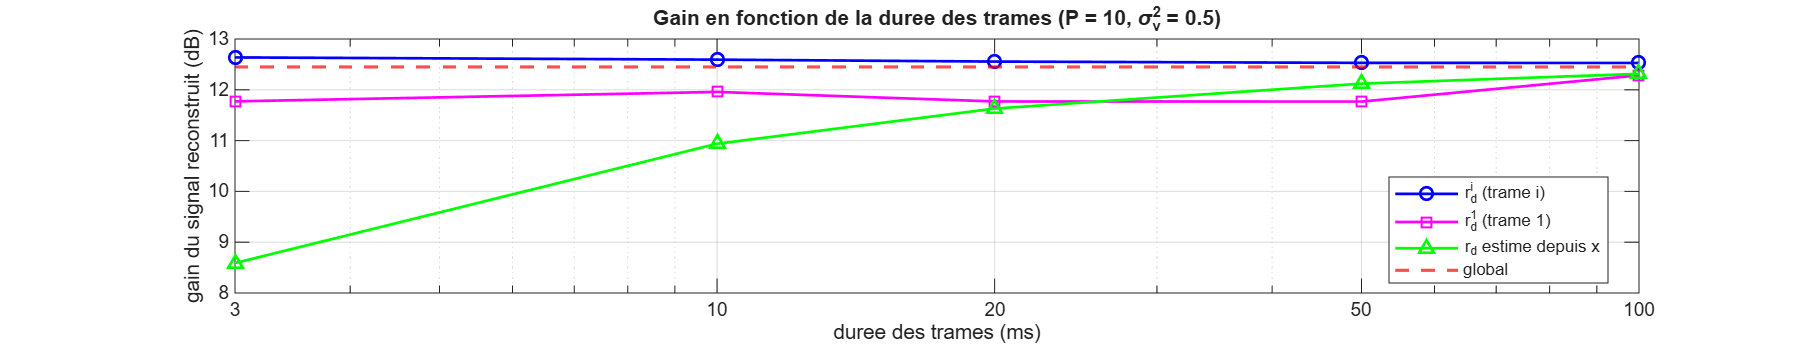
\includegraphics[width=\linewidth]{p3_qf_gain_duree}

  \medskip
  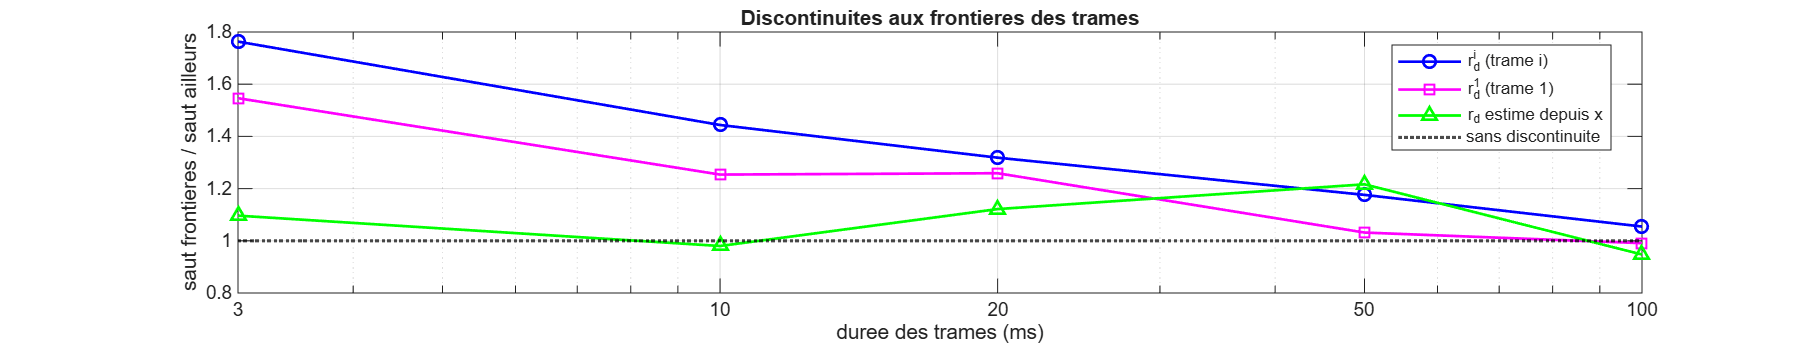
\includegraphics[width=\linewidth]{p3_qf_saut_duree}
  \caption{En haut : gain du signal reconstruit en fonction de la durée des trames, pour les trois façons d'obtenir $\mathbf{r}_{d}$. En bas : rapport saut aux frontières / saut moyen ($P=10$, $\sigma_v^2=0.5$).}
\end{figure}

\begin{figure}[H]
  \centering
  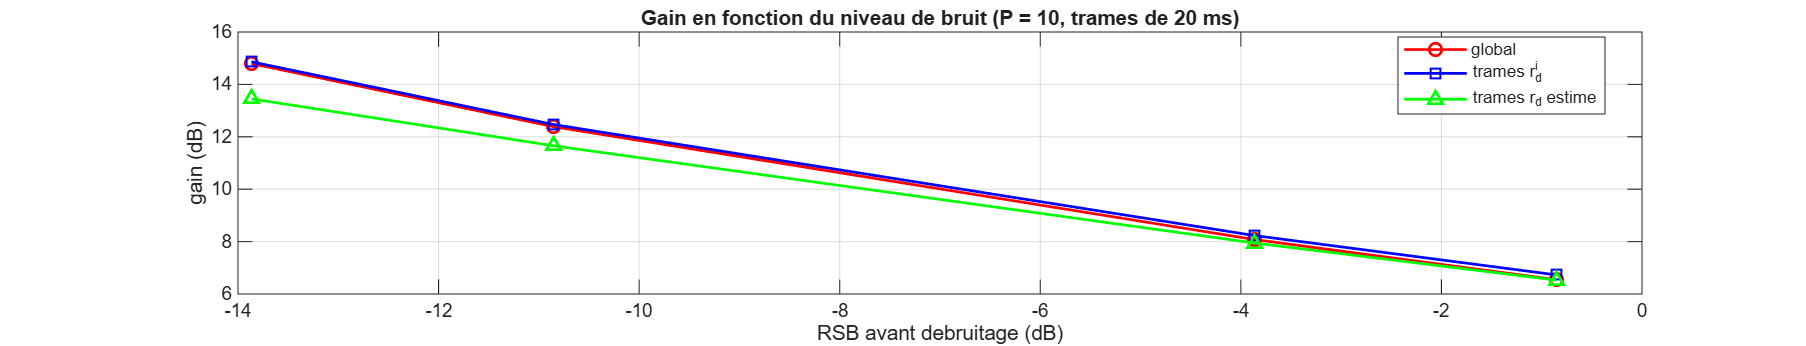
\includegraphics[width=\linewidth]{p3_qf_gain_bruit}

  \medskip
  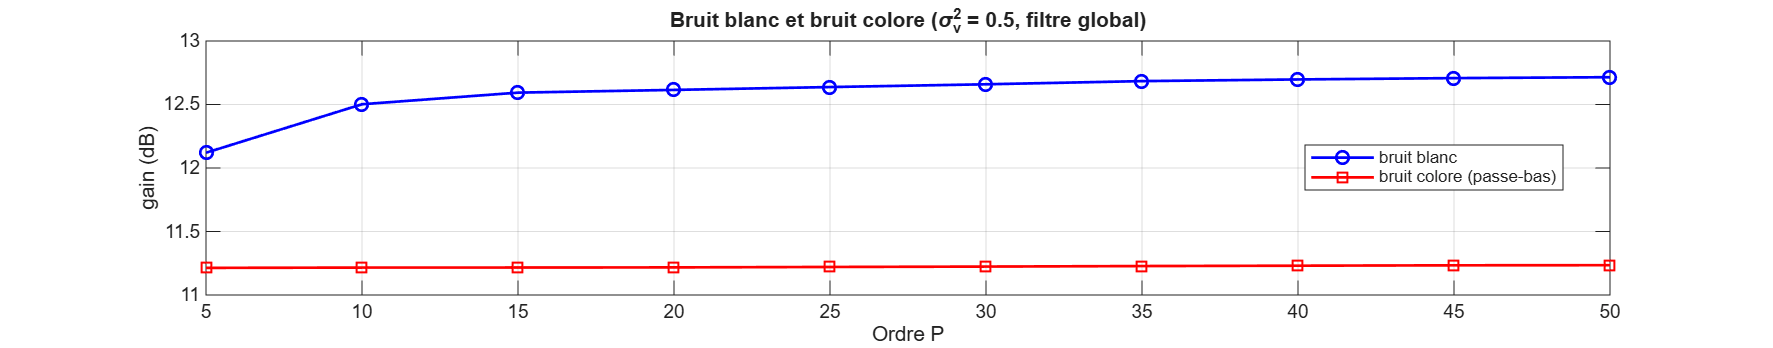
\includegraphics[width=\linewidth]{p3_qf_bruit_colore}
  \caption{En haut : gain en fonction du RSB avant débruitage ($P=10$, trames de $20$~ms). En bas : gain du filtre global en fonction de $P$ pour un bruit blanc et un bruit coloré de même puissance ($\sigma_v^2=0.5$).}
\end{figure}

\begin{interpretation}
\begin{itemize}
  \item \textbf{Durée des trames.} Avec $\mathbf{r}^i_{d}$, le gain ne dépend presque pas de la durée ($12.60$~dB à $3$~ms, $12.53$~dB à $100$~ms, toujours au-dessus du global : $12.45$~dB), mais les discontinuités diminuent nettement (rapport $1.76$ à $3$~ms, $1.32$ à $20$~ms, $1.05$ à $100$~ms). À l'écoute, les trames de $20$~ms sonnent nettement mieux que celles de $3$~ms : $6.7$ fois moins de frontières, des sauts plus faibles et des filtres estimés sur $882$ échantillons au lieu de $132$. Avec $\mathbf{r}^1_{d}$, le gain reste vers $11.8$~dB et ne remonte qu'à $100$~ms ($12.28$~dB), quand la trame 1 devient représentative.
  \item \textbf{Signal propre indisponible.} L'estimation $r_d(k)=r_x(k)-\sigma_v^2\delta(k)$ dépend fortement de la durée des trames : $8.59$~dB à $3$~ms, $11.63$~dB à $20$~ms, $12.31$~dB à $100$~ms (presque le global). Sur une trame courte, l'erreur d'estimation de $r_x(k)$ est amplifiée par la soustraction de $\sigma_v^2$. Compromis retenu : trames de $20$ à $50$~ms.
  \item \textbf{Niveau de bruit.} Le gain croît avec le bruit : $6.55$~dB pour $\sigma_v^2=0.05$ ($\mathrm{RSB}_{\mathrm{av}}=-0.86$~dB) à $14.79$~dB pour $\sigma_v^2=1$ ($\mathrm{RSB}_{\mathrm{av}}=-13.87$~dB), effet mécanique déjà vu en (c) et (d). Les trames avec $\mathbf{r}^i_{d}$ gardent $0.1$ à $0.2$~dB d'avance sur le global ; l'estimation sans signal propre perd jusqu'à $1.3$~dB à fort bruit.
  \item \textbf{Bruit coloré.} Pour $P=10$, le gain passe de $12.50$~dB (bruit blanc) à $11.22$~dB (bruit coloré), et augmenter $P$ n'apporte plus rien (courbe plate vers $11.2$~dB, contre $12.7$~dB en bruit blanc). Le bruit passe-bas occupe la même bande que le signal (les vagues) : un filtre linéaire ne peut pas séparer deux composantes de même bande, quel que soit son ordre.
\end{itemize}
\end{interpretation}
